\section{音声信号処理}
音声にはフォルマントや基本周波数(ピッチ)など,様々な周波数的な特徴が存在している.フォルマントは母音や子音を知覚するため,ピッチはアクセントやイントネーションを表現するために重要なものである.このような音声信号の持つ複雑さから,時間波形のままその特徴を分析することは困難である.これに対し,本節では音声の特徴を捉えやすくするための信号処理について説明する.

\subsection{音声のフーリエ変換}
音声の時間波形に対して,周波数領域での情報を得るためにはフーリエ変換(Fourier Transform)を使用する.特に,音声はマイクロフォンで収録され,コンピュータ内で処理されることが多い.この時,音声はアナログ信号ではなく,サンプリング周波数と量子化ビット数に従って離散化されたデジタル信号として扱われる.このような場合,離散信号に対してのフーリエ変換である離散フーリエ変換(discrete Fourier transform; DFT)が用いられる.また,信号の系列長をゼロパディングして2の冪乗の長さに調整することで,計算量を抑えた高速フーリエ変換(fast Fourier transform; FFT)を用いることができる.

離散信号を$x[n]$,それに対するフーリエ変換を$X[k]$とする.ここで,nはサンプルのインデックス,kは周波数インデックスである.$X[k]$は複素数であり,以下のように極座標表示することができる.
\begin{align}
    X[k] & = \mathrm{Re}\lr{X[k]} + j\mathrm{Im}\lr{X[k]} \\
         & = |X[k]|e^{j\angle\mathrm{X[k]}}
\end{align}
ここで,$|X[k]|$は振幅特性(振幅スペクトル),$\angle\mathrm{X[k]}$は位相特性(位相スペクトル)であり,
\begin{gather}
    |X[k]| = \sqrt{\mathrm{Re}\lr{X[k]}^{2} + \mathrm{Im}\lr{X[k]}^{2}} \\
    \angle\mathrm{X[k]} = \tan^{-1} \frac{\mathrm{Im}\lr{X[k]}}{\mathrm{Re}\lr{X[k]}}
\end{gather}
と表される.また,$|X[k]|^2$はパワースペクトルと呼ばれる.これにより,信号中にどのような周波数成分がどれくらい含まれているかを調べることができる.しかし,音声はフォルマントやピッチが時々刻々と変化するため,信号全体に対して直接フーリエ変換を適用したとしても有用な結果が得られない.このような音声の持つ非定常性の問題に対して,十分短い時間幅においては信号の定常性が成り立つという仮定のもと,短時間フーリエ変換(short-time Fourier transform; STFT)が用いられる.STFTでは,音声信号に対して窓関数による窓処理を適用し,短時間に区切られた信号それぞれに対してDFTを適用する.ここで,窓処理とはある特定の窓関数と音声信号を時間領域でかけ合わせることであり,窓関数の時間幅を窓長という.また,窓関数を時間方向にシフトするときの時間幅をシフト幅という.STFTには時間分解能と周波数分解能の間に不確定性が存在し,両者の間にトレード・オフの関係がある.窓長が長い場合には周波数分解能が向上する一方,時間分解能が低下する.窓長が短い場合にはその逆となる.音声信号$x[n]$のSTFTを時刻$j$,周波数インデックスを$k$として$X[j, k]$と表すと,$X[j, k]$は時間周波数領域における複素数となる.これを複素スペクトログラムと呼ぶ.また,$|X[j, k]|$を振幅スペクトログラム,$\angle\mathrm{X[j, k]}$を位相スペクトログラム,
$|X[j, k]|^{2}$をパワースペクトログラムと呼ぶ.「小さな鰻屋に,熱気のようなものがみなぎる」と発話した音声に対し,窓関数としてハニング窓を用いた上で,複数の窓長・シフト幅によって計算した対数パワースペクトログラムを,図~\ref{sec2:fig:log_power_spectrograms}に示す.窓長が100msと長い場合には周波数分解能が高いが,時間分解能が低下することでスペクトルの時間変化が滑らかでないことがわかる.一方,窓長が12.5msと短い場合には時間分解能が高いが,周波数分解能が低下することでスペクトルがぼやけていることがわかる.これが窓長に対する時間分解能と周波数分解能とトレード・オフであり,窓長25msや50msが程よいパラメータであることがわかる.
\begin{figure}[tb]
    \centering
    \begin{subfigure}[b]{0.48\textwidth}
        \centering
        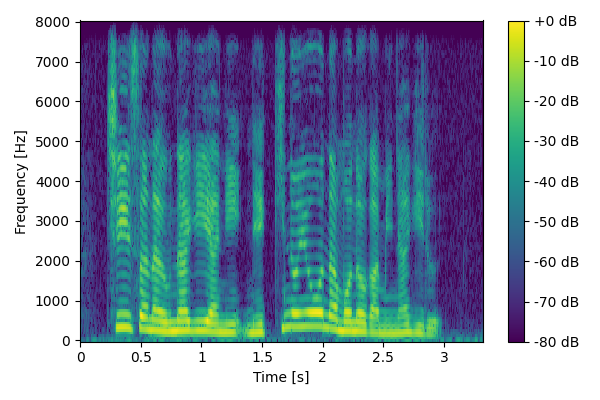
\includegraphics[width=\textwidth]{./figure/sec2/spectrogram_1.png}
        \caption{窓長12.5ms,シフト幅5ms}
        \label{sec2:fig:spectrogram1}
    \end{subfigure}
    \begin{subfigure}[b]{0.48\textwidth}
        \centering
        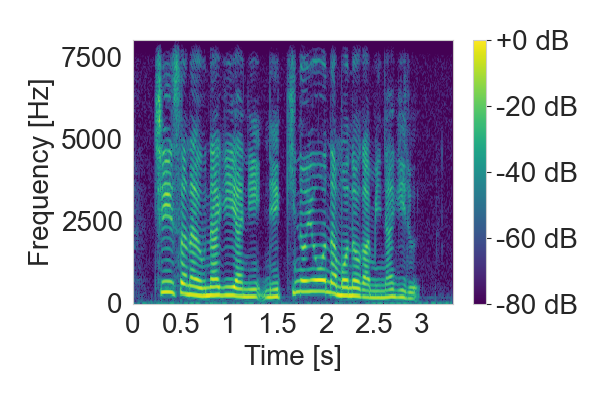
\includegraphics[width=\textwidth]{./figure/sec2/spectrogram_2.png}
        \caption{窓長25ms,シフト幅10ms}
        \label{sec2:fig:spectrogram2}
    \end{subfigure}

    \vspace{0.5cm}

    \begin{subfigure}[b]{0.48\textwidth}
        \centering
        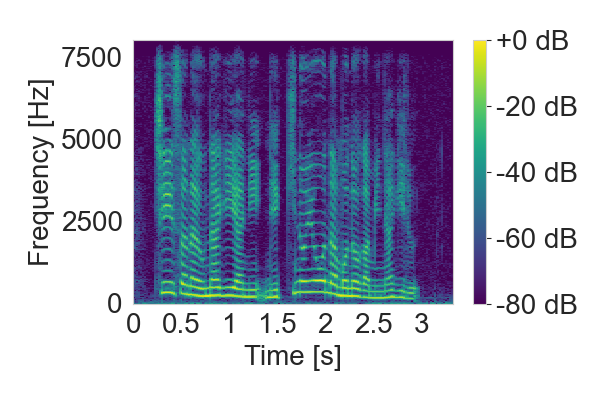
\includegraphics[width=\textwidth]{./figure/sec2/spectrogram_4.png}
        \caption{窓長50ms,シフト幅20ms}
        \label{sec2:fig:spectrogram3}
    \end{subfigure}
    \begin{subfigure}[b]{0.48\textwidth}
        \centering
        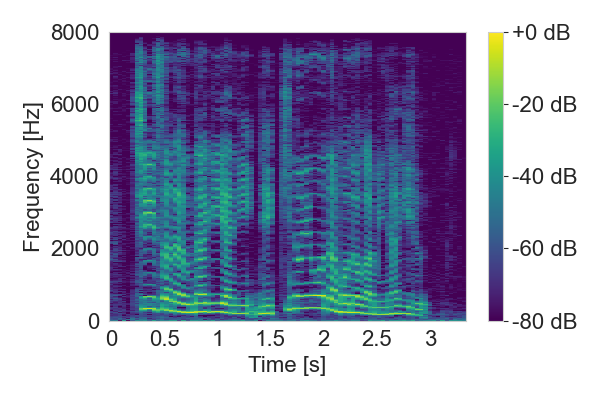
\includegraphics[width=\textwidth]{./figure/sec2/spectrogram_8.png}
        \caption{窓長100ms,シフト幅40ms}
        \label{sec2:fig:spectrogram4}
    \end{subfigure}
    \caption{「小さな鰻屋に,熱気のようなものがみなぎる」と発話した音声から計算された対数パワースペクトログラム}
    \label{sec2:fig:log_power_spectrograms}
\end{figure}

\subsection{メルスペクトログラム}
メルスペクトログラムは,パワースペクトログラムを人間の聴感特性を考慮したメル尺度に変換することによって得られる.周波数軸をメル尺度に変換する際,以下の式を用いる.
\begin{equation}
    \text{Mel}\lr{f} = 2595\log_{10} \lr{1 + \frac{f}{700}}
\end{equation}
メル尺度は,$\SI[]{1000}{Hz}$,$\SI[]{40}{dB}$の純音を$\SI[]{1000}{mel}$とする比率尺度である.メル尺度を用いることにより,低い周波数ほど細かく,高い周波数ほど荒い特徴量になる.メルスペクトログラムは,パワースペクトログラムに対してメルフィルタバンクを適用することによって得られる.メルフィルタバンクの数は任意に決定できるパラメータであり,メルスペクトログラムの周波数方向の次元はこれに一致する.音声合成においては,音声のサンプリング周波数を$\SI[]{16}{kHz}$とするとき,メルフィルタバンクの数を80とし,$\SI[]{8000}{Hz}$までの帯域に対して適用することが多い.「小さな鰻屋に,熱気のようなものがみなぎる」と発話した音声に対し,窓関数にハニング窓を用い,窓長25ms,シフト幅10msとしてパワースペクトログラムを計算した上で,80次元のメルフィルタバンクを適用して得られた対数メルスペクトログラムを,図~\ref{sec2:fig:melspectrogram}に示す.
\begin{figure}[bt]
    \centering
    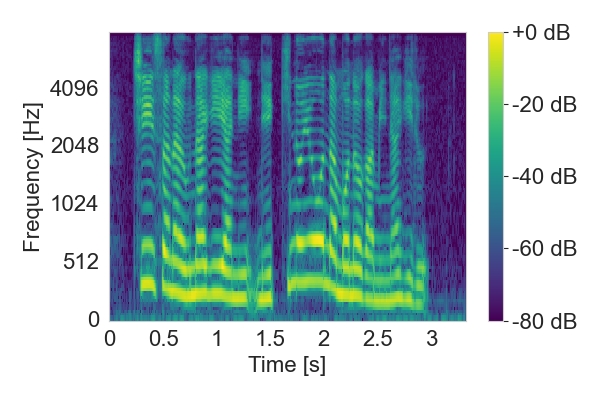
\includegraphics[height=70mm]{./figure/sec2/melspectrogram.png}
    \caption{「小さな鰻屋に,熱気のようなものがみなぎる」と発話した音声に対する対数メルスペクトログラム}
    \label{sec2:fig:melspectrogram}
\end{figure}